\section{Research Problems}
In this section,I introduce three motivating tasks which this thesis aims to solve and briefly discuss my proposed approaches. The first task is \textit{Personalized Community Detection}, in which communities with different resolutions are formed given user information need. The second task is \textit{Cross-Graph Community Detection}, in which I detect pairwise user community closeness in sparse graphs by leveraging propagated information from external graphs. The third task is \textit{Community-Aware Dynamic Product Summarization}, in which community  is applied as supportive information to generate temporal product summarizations across different time periods. Details of my proposed models, along with extensive experiments and discussions, are introduced in the following chapters.

\subsection{Personalized Community Detection}
From a user-centric viewpoint, the ideal communities should provide a high-resolution partition in areas of the graph relevant to the user’s needs and a coarse partition on the remaining areas so as to best respond to the user’s needs (which can be formulated as a ``query'') in concentrated areas while leaving irrelevant areas less precisely specified. 

For instance, in Figure \ref{fig:example}, two different scholars in \textit{education} and \textit{data mining} domains, respectively, may consume the same scholarly graph differentlybecause they may need more detailed community exploration in their own domains whereas generalized community information is sufficient in irrelevant domains. For instance, a \textit{data mining} scholar may need more detailed communities in areas such as deep learning, graph mining, and Bayesian analysis, but for an \textit{education} researcher it may suffice to generalize these as computer science or even just science.

\begin{figure}
	% \setlength{\belowcaptionskip}{-10pt}
	\center
	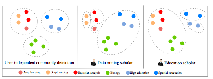
\includegraphics[width=0.8\columnwidth]{img/chapter3/example.pdf} 
	\caption{An example of personalized community detection on a scholarly graph} 
	\label{fig:example}
\end{figure}  

To solve this problem, I propose a \textbf{g}enetic \textbf{P}ersonalized \textbf{C}ommunity \textbf{D}etection (gPCD) model with an offline and an online step to efficiently cope with the time complexity issue in personalized community detection.  Details of the model structure are given in Chapter \ref{ch:personalized}.

\subsection{Cross-Graph Community Detection}
For a vulnerable graph with sparse connectivity, however, existing community detection algorithms can hardly probe enough information to optimize the community structure. Unfortunately, in real cyberspace this is a very common problem: while a handful of giant players (e.g., Google, Facebook, and Amazon) maintain high-quality graphs, thousands of apps are suffering from a “cold-start” problem in this area. If many users are isolated because of data sparseness, I can hardly determine any community information. 

To cope with this challenge, in this thesis I propose a novel research problem: Cross-Graph Community Detection. The idea is based on the fact that an increasing number of small apps are utilizing user identity information inherited from giant providers; for instance, users can easily log in to a large number of new apps using Facebook and Google ID. In such an ecosystem, the large main graph can provide critical information to enlighten community detection in many small sparse graphs. Figure \ref{fig:c4_example}depicts an example in which the Cooking and Cosmetic apps inherit important topological information from the main Amazon graph for enhanced community detection.

\begin{figure}  
	% \advance\leftskip-1cm 
	% \hspace*{0.25cm} 
	\centering
	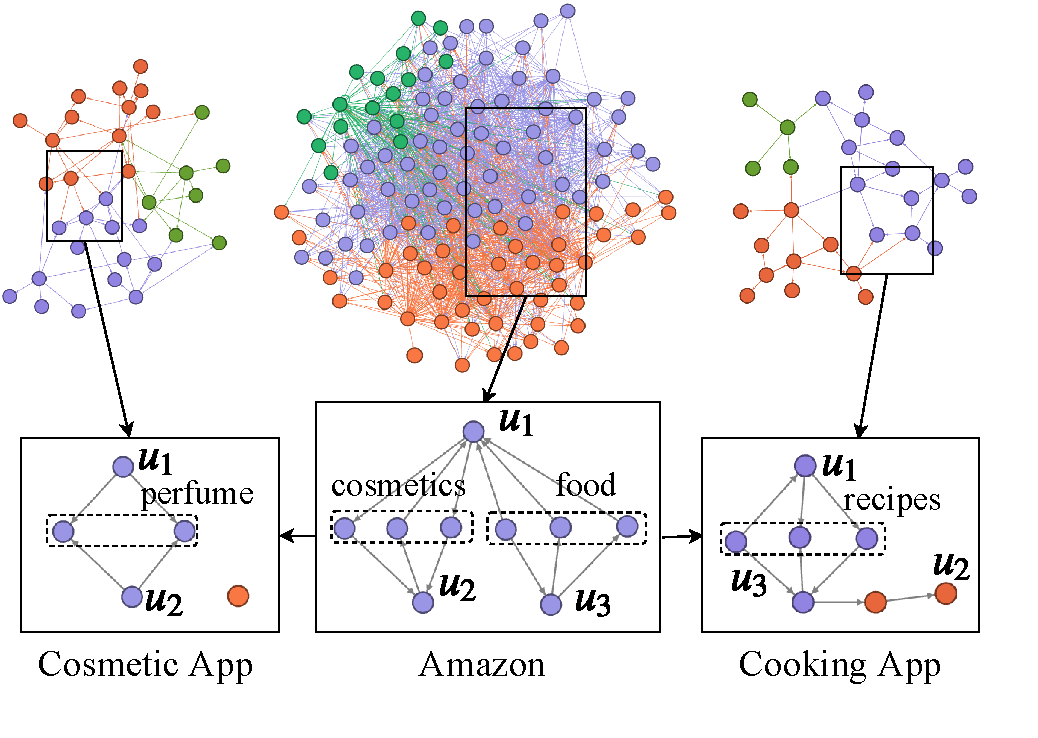
\includegraphics[width=0.8\columnwidth]{img/chapter4/example.pdf}
	%  \vspace{-1em}
	\caption{The Amazon graph is a main shopping graph while the Cosmetic App and the Cooking App are two small sparse graphs. Those graphs share mutual users in which three of them are selected to demonstrate their behaviors. Node colors indicate their related communities. }
	\label{fig:c4_example}
	%   \vspace{-1em}
\end{figure}

Inspired by the foregoing discussion, I propose an innovative \textit{Pairwise Cross-graph Community Detection} (PCCD) model for enhanced sparse graph user community detection. Specifically, given user $u_i$ and its associated triplet $\langle u_{i},u_{j},u_{k}\rangle$, I aim to predict the pairwise community relationships, e.g., compared with user $u_{k}$, does user $u_{j}$ have closer, similar or farther community closeness to user $u_i$? The details of this model structure are mentioned in Chapter \ref{ch:cross-graph}.

\subsection{Community-Aware Dynamic Product Summarization}
Product communities can implicitly reflect product characteristics. Therefore, understanding product communities and tracking their changes in a timely manner can support better decision-making for commercial purposes, such as informing online retailers in creating timely sales plans. Therefore, the \textit{Dynamic Community-Aware Product Summarization} task is of great importance. Such summarization not only indicates products’ dynamic membership changes but also utilizes these changes to depict product characteristics in readable contexts for easier interpretation.

\begin{figure}  
	% \advance\leftskip-1cm 
	\centering
	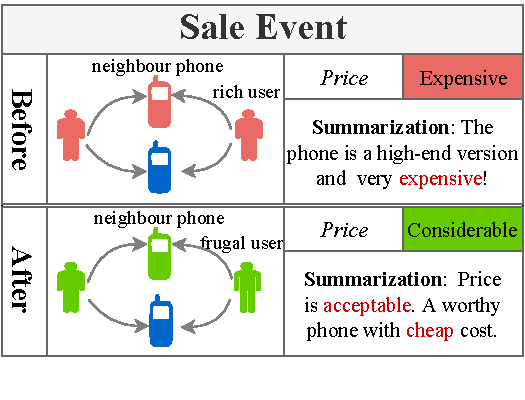
\includegraphics[width=0.8\columnwidth]{img/chapter5/example.pdf}
	% 	\vspace{-1em}
	\caption{An example to illustrate how to dynamically detect communities and select within-community neighbor products (red phone $\rightarrow$ green phone) for depicting current product (blue phone) characteristic change before \& after a sale event from user behaviors.}
	\label{fig:c5_example}
	% 	\vspace{-1.5em} 
\end{figure}

However, existing generative models relying on reviews inevitably face the sparsity issue: few products can gain enough reviews in a short time to depict the product’s temporal characteristics. User behaviors, on the other hand, are abundant and highly related to the product’s nature. Therefore, instead of review-based product summarization, I aim to generate community-aware product summarization in a dynamic manner. These approaches share the same goal but have huge differences in terms of proposed models. Review-based summarization directly runs a sequence-to-sequence model to generate product summarization by simply leveraging review context information. A community-aware product summarization, however, is generated from within-community neighbor product reviews. This means that it is a two-step approach, requiring both community detection and summarization generation.

As Figure \ref{fig:c5_example} depicts, when a sale event on a high-end phone brings frugal users' instant \textit{clicks}, behavior-based algorithms can immediately consume this information and locate updated within-community neighbor products (red phone $\rightarrow$ green phone) whose sufficient reviews help to update the product (blue phone) summarization. For review-based approaches, accumulating enough reviews to characterize this dynamic change may take a longer time. 

In the end,  I propose a  \textbf{B}ehavior based \textbf{D}ynamic \textbf{S}ummarization (BDS) model to accommodate user behavior for dynamic product summarization. The proposed model uses learned communities as a criteria to select neighbor products via a reinforcement approach, where textual review information is used to generate target product summarizations in a timely manner. Details of the model structure are given in Chapter \ref{ch:community-aware}.